\appendix

\section{System Architecture Details}

\begin{lstlisting}[caption={Project directory structure}, label={lst:project_structure}, style=tree]
project/
|-- CMakeLists.txt
|-- data/
|   |-- in.ppm
|   `-- out.ppm
|-- src/
|   |-- main/
|   |   `-- main.cpp
|   |-- image/
|   |   |-- image_gray.h/.cpp
|   |   `-- colorspace.h/.cpp
|   |-- io/
|   |   |-- ppm_reader.h/.cpp
|   |   |-- ppm_writer.h/.cpp
|   |   `-- token_reader.h/.cpp
|   |-- ops/
|   |   |-- denoise_median.h/.cpp
|   |   |-- background_estimate.h/.cpp
|   |   |-- background_remove.h/.cpp
|   |   |-- contrast_stretch.h/.cpp
|   |   |-- threshold_otsu.h/.cpp
|   |   |-- threshold_sauvola.h/.cpp
|   |   |-- threshold_nick.h/.cpp
|   |   |-- threshold_su.h/.cpp
|   |   |-- threshold_proposed.h/.cpp
|   |   |-- morphology.h/.cpp
|   |   `-- border_cleanup.h/.cpp
|   `-- util/
|       |-- args_parser.h/.cpp
|       |-- logging.h/.cpp
|       |-- timing.h/.cpp
|       `-- clamp.h
`-- tests/
    |-- io/
    |   `-- test_ppm_io.cpp
    `-- ops/
        |-- test_otsu.cpp
        |-- test_sauvola.cpp
        `-- test_median.cpp
\end{lstlisting}


\section{Results of The Implemented Binarization Methods}

\begin{figure}[H]
\centering
\small
\renewcommand{\arraystretch}{1.0}
\setlength{\tabcolsep}{3pt}

\begin{tabular}{c c c}

\textbf{Method} & \textbf{Without Preprocessing} & \textbf{With Preprocessing} \\[0.3em]

\hline \\[-0.5em]

Original &
\multicolumn{2}{c}{
\includegraphics[width=0.25\textwidth]{images/test.jpg}} \\[0.4em]

\hline \\[-0.5em]

Otsu &

\includegraphics[width=0.25\textwidth]{images/otsu.png} &

\includegraphics[width=0.25\textwidth]{images/otsu_with_preprosseing.png} \\[0.4em]

\hline \\[-0.5em]

Nick &
--- &
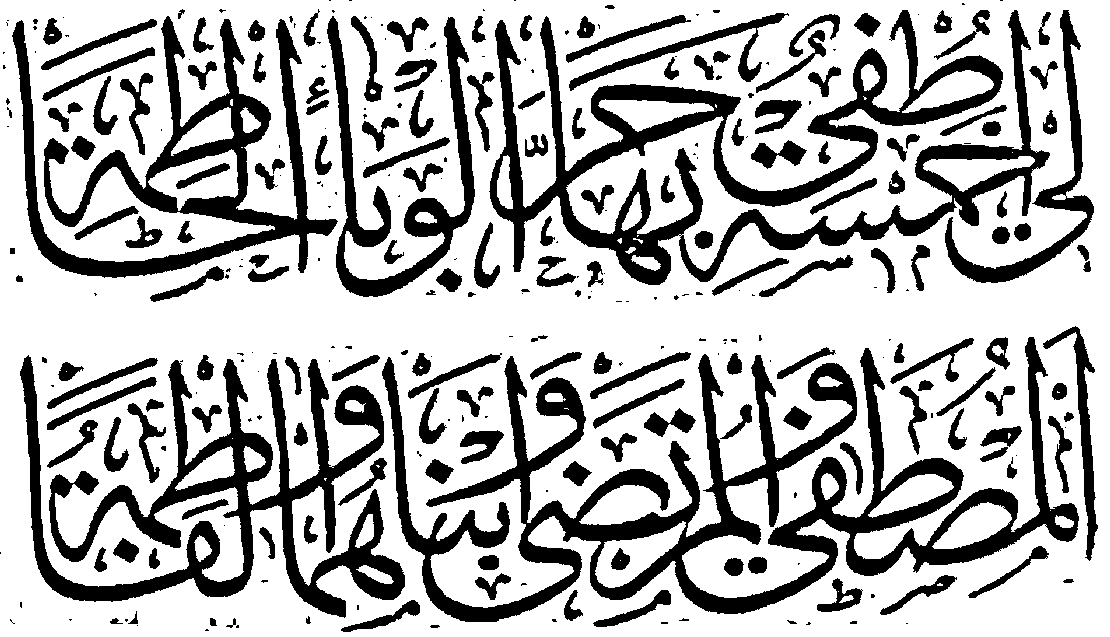
\includegraphics[width=0.25\textwidth]{images/nick_with_preprosseing.png} \\[0.4em]

\hline \\[-0.5em]

Sauvola &

\includegraphics[width=0.25\textwidth]{images/sauvola.png} &
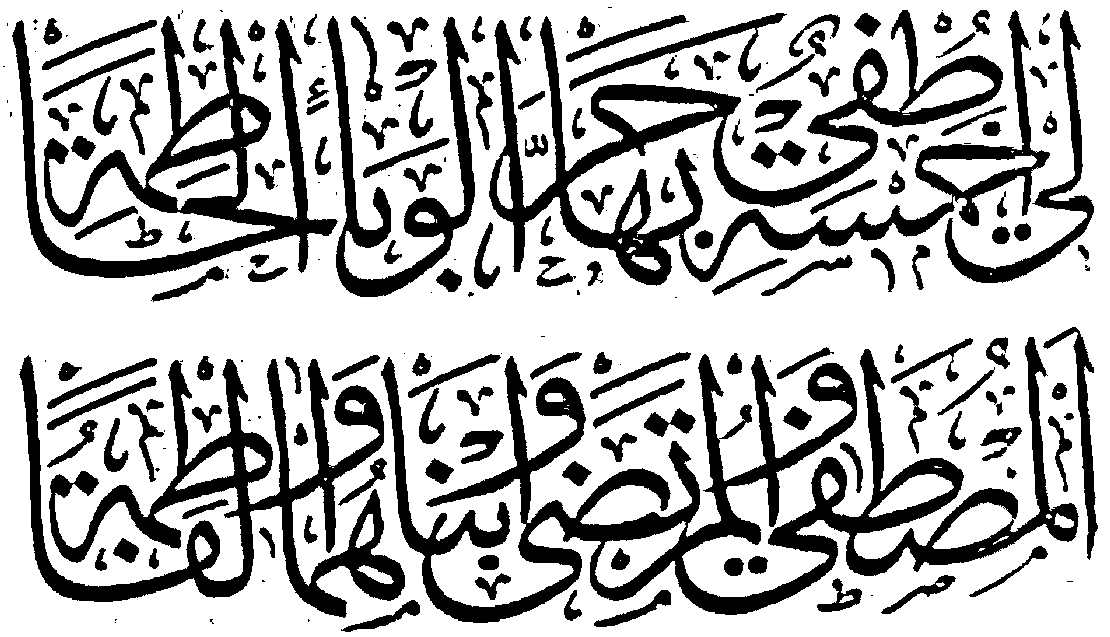
\includegraphics[width=0.25\textwidth]{images/sauvola_with_preprosseing.png} \\[0.4em]

\hline \\[-0.5em]

Su &

\includegraphics[width=0.25\textwidth]{images/su.png} &

\includegraphics[width=0.25\textwidth]{images/su_with_preprosseing.png} \\[0.4em]

\hline \\[-0.5em]

Proposed &

\includegraphics[width=0.25\textwidth]{images/proposed copy.png} &
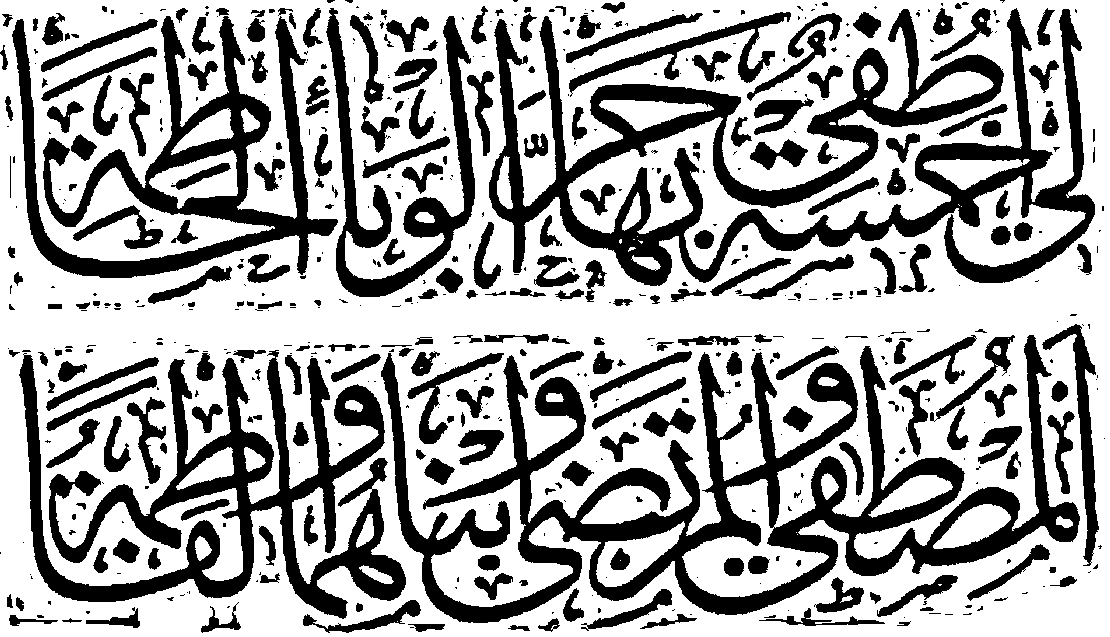
\includegraphics[width=0.25\textwidth]{images/proposed_with_preprosseing.png} \\[0.4em]

\hline

\end{tabular}

\caption{Binarization results of all implemented methods, without and with preprocessing (contrast stretch percentile).}

\label{tab:binarization-results}

\end{figure}